% ===================================================================
%  Week 12 — Session 1: Image features & the recognition pipeline
% ===================================================================
\documentclass[10pt,aspectratio=169]{beamer}
% ===================================================================
%  Shared Beamer preamble for "Practical Image Processing"
%  English slides. Compile with pdfLaTeX.
% ===================================================================

\usetheme{metropolis}
\usepackage[T1]{fontenc}
\usepackage[utf8]{inputenc}
\usepackage{lmodern}
\usepackage{listings}
\usepackage{tcolorbox}
\usepackage{fontawesome5}
\usepackage{booktabs}
\usepackage{amsmath,amssymb}
\usepackage{tikz}
\usepackage{pgfplots}
\pgfplotsset{compat=1.17}
\usetikzlibrary{arrows.meta,positioning,shapes.geometric,fit,backgrounds,matrix}
\tcbuselibrary{skins,breakable}

% ---- Palette --------------------------------------------------------
\definecolor{coursePrimary}{HTML}{1B4965}   % deep blue
\definecolor{courseAccent}{HTML}{E76F51}    % coral
\definecolor{courseGood}{HTML}{2A9D8F}      % teal
\definecolor{courseBad}{HTML}{C0392B}       % red
\definecolor{courseInfo}{HTML}{2980B9}      % blue
\definecolor{codeBg}{HTML}{F5F6FA}
\definecolor{codeKw}{HTML}{8E44AD}
\definecolor{codeStr}{HTML}{2A9D8F}
\definecolor{codeCom}{HTML}{7F8C8D}

\setbeamercolor{frametitle}{bg=coursePrimary}
\setbeamercolor{progress bar}{fg=courseAccent}
\setbeamercolor{alerted text}{fg=courseAccent}
\metroset{block=fill,sectionpage=progressbar,numbering=fraction}

% ---- Code listings (Python is built into listings) -----------------
\lstdefinestyle{course}{
  backgroundcolor=\color{codeBg},
  basicstyle=\ttfamily\scriptsize,
  keywordstyle=\color{codeKw}\bfseries,
  stringstyle=\color{codeStr},
  commentstyle=\color{codeCom}\itshape,
  numberstyle=\tiny\color{codeCom},
  numbers=left, numbersep=6pt,
  showstringspaces=false, breaklines=true, breakatwhitespace=true,
  tabsize=4, columns=fullflexible,
  frame=single, framesep=4pt, rulecolor=\color{gray!30},
  keepspaces=true, upquote=true, language=Python,
}
\lstset{style=course}
\lstdefinelanguage{bash}{
  keywords={cd,pip,python,venv,source,import}, sensitive=true,
  morecomment=[l]{\#}, morestring=[b]', morestring=[b]",
}

% ---- Reusable callout boxes ----------------------------------------
\newtcolorbox{goodbox}[1][Good practice]{colback=courseGood!8,colframe=courseGood,
  fonttitle=\bfseries,title={\faCheck~#1},boxrule=0.6pt,left=4pt,right=4pt,top=3pt,bottom=3pt}
\newtcolorbox{badbox}[1][Pitfall]{colback=courseBad!8,colframe=courseBad,
  fonttitle=\bfseries,title={\faTimes~#1},boxrule=0.6pt,left=4pt,right=4pt,top=3pt,bottom=3pt}
\newtcolorbox{infobox}[1][Note]{colback=courseInfo!8,colframe=courseInfo,
  fonttitle=\bfseries,title={\faInfoCircle~#1},boxrule=0.6pt,left=4pt,right=4pt,top=3pt,bottom=3pt}
\newtcolorbox{mathbox}[1][Math]{colback=coursePrimary!6,colframe=coursePrimary,
  fonttitle=\bfseries,title={\faCalculator~#1},boxrule=0.6pt,left=4pt,right=4pt,top=3pt,bottom=3pt}

\newcommand{\keyidea}[1]{\begin{alertblock}{Key idea}#1\end{alertblock}}
\newcommand{\term}[1]{\textbf{\color{coursePrimary}#1}}
\newcommand{\code}[1]{\lstinline[basicstyle=\ttfamily\small]|#1|}

% ---- A helper to draw a small pixel grid, cells shaded by value ----
% \pixelgrid{ {10,20,120,200,240}, {30,60,130,180,230}, ... }
\newcommand{\pixelgrid}[1]{%
  \begin{tikzpicture}[font=\scriptsize,scale=0.6]
    \foreach \row [count=\ry] in {#1} {
      \foreach \val [count=\cx] in \row {
        \draw[gray,fill=coursePrimary!8] (\cx,-\ry) rectangle ++(1,-1);
        \node at (\cx+0.5,-\ry-0.5) {\val};
      }
    }
  \end{tikzpicture}}


\title{From Features to Machine Learning}
\subtitle{Week 12 — Session 1: Image features \& the recognition pipeline}
\author{Practical Image Processing}
\date{Lecture 12.1 \textbullet\ 60--70 min}

\begin{document}

\maketitle

\begin{frame}{A turning point in the course}
  \begin{columns}[T]
    \begin{column}{0.58\textwidth}
      \begin{itemize}
        \item Weeks 1--11: \emph{we} designed every step (filters, edges, corners, warps).
        \item \alert{Now:} we let the computer \emph{learn} the decision from labelled examples.
        \item The bridge: turn an image into a \term{feature vector}, then train a \term{classifier}.
      \end{itemize}
    \end{column}
    \begin{column}{0.42\textwidth}
      \begin{alertblock}{Today's real task}
        Classify Iranian car models (206 / 405 / Dena) from \term{HOG} features — using your
        \code{E:/data} images.
      \end{alertblock}
    \end{column}
  \end{columns}
\end{frame}

\begin{frame}{Where Session 1 stops}
  \begin{itemize}
    \item \textbf{Session 1 (today):} how to turn an image into a \emph{good} feature vector, and what a classifier is.
    \item \textbf{Session 2 (next):} training, honest evaluation, overfitting, and the limits of hand-crafted features.
  \end{itemize}
  \keyidea{You cannot fix a bad classifier with more training. Everything starts with the features. Today is about features.}
\end{frame}

\begin{frame}{Roadmap}\tableofcontents\end{frame}

% ==================================================================
\section{The recognition pipeline}
% ==================================================================

\begin{frame}{The classic recognition pipeline}
  \begin{center}
  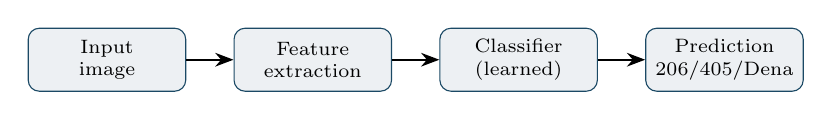
\begin{tikzpicture}[font=\scriptsize,node distance=6mm,
      box/.style={draw=coursePrimary,fill=coursePrimary!8,rounded corners,
        minimum height=8mm,minimum width=20mm,align=center},
      >=Stealth]
    \node[box] (img) {Input\\image};
    \node[box,right=of img] (feat) {Feature\\extraction};
    \node[box,right=of feat] (clf) {Classifier\\(learned)};
    \node[box,right=of clf] (pred) {Prediction\\206/405/Dena};
    \draw[->,thick] (img) -- (feat);
    \draw[->,thick] (feat) -- (clf);
    \draw[->,thick] (clf) -- (pred);
  \end{tikzpicture}
  \end{center}
  \begin{enumerate}
    \item \term{Input image} $\rightarrow$
    \item \term{Feature extraction} (turn pixels into a compact vector) $\rightarrow$
    \item \term{Classifier} (a learned function: vector $\rightarrow$ label) $\rightarrow$
    \item \term{Prediction}.
  \end{enumerate}
  \keyidea{Until $\sim$2012, essentially all recognition worked this way. The features were hand-designed; only the classifier was learned.}
\end{frame}

\begin{frame}{Why not feed raw pixels?}
  \begin{itemize}
    \item A $96\times96$ image is $9216$ numbers — huge, and every shift/lighting change moves them all.
    \item Raw pixels are not \term{invariant}: the same car, moved 5\,px, looks ``different''.
    \item \term{Features} (HOG, colour histograms, ORB) compress the image into a stable, meaningful vector.
  \end{itemize}
  \begin{mathbox}
    Shift a $96\times96$ image by one pixel: almost all $9216$ values change, yet it is the \emph{same} car.
    A raw-pixel distance would call it far away. Good features must not.
  \end{mathbox}
\end{frame}

\begin{frame}{The curse of dimensionality}
  \begin{columns}[T]
    \begin{column}{0.56\textwidth}
      \begin{itemize}
        \item In $9216$ dimensions, ``nearest neighbour'' becomes almost meaningless — distances all look similar.
        \item You need exponentially more examples to fill a high-dimensional space.
        \item Features cut $9216 \rightarrow$ a few hundred meaningful numbers.
      \end{itemize}
    \end{column}
    \begin{column}{0.44\textwidth}
      \begin{badbox}[More dimensions than samples]
        126 training images but a $9216$-D pixel vector? The model has enough freedom to memorize noise.
      \end{badbox}
    \end{column}
  \end{columns}
\end{frame}

\begin{frame}{What makes a good feature}
  \begin{itemize}
    \item \term{Invariant} to nuisances: small shifts, lighting, minor rotation.
    \item \term{Discriminative}: different classes land in different regions.
    \item \term{Compact}: a few hundred numbers, not ten thousand.
  \end{itemize}
  \begin{mathbox}
    Good features make classes \term{separable}: similar things land near each other, different things land apart —
    in a space small enough to learn a boundary.
  \end{mathbox}
\end{frame}

% ==================================================================
\section{Gradients: the raw material of HOG}
% ==================================================================

\begin{frame}{Gradients recap — where edges point}
  \begin{columns}[T]
    \begin{column}{0.5\textwidth}
      \begin{itemize}
        \item Recall the gradient $\nabla I = (I_x, I_y)$ from the edges week.
        \item \term{Magnitude} $=\sqrt{I_x^2+I_y^2}$ says \emph{how strong} the edge is.
        \item \term{Orientation} $=\arctan(I_y/I_x)$ says \emph{which way} it points.
      \end{itemize}
      HOG throws away the exact pixels and keeps only \emph{orientation}, weighted by magnitude.
    \end{column}
    \begin{column}{0.5\textwidth}
      \begin{center}
      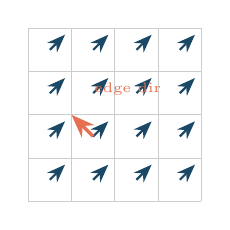
\begin{tikzpicture}[scale=0.55,>=Stealth,font=\scriptsize]
        \draw[step=1,gray!40] (0,0) grid (4,4);
        \foreach \x in {0,...,3}{\foreach \y in {0,...,3}{
          \draw[->,coursePrimary,thick] (\x+0.5,\y+0.5) -- ++(0.35,0.35);}}
        \draw[->,courseAccent,very thick] (1.5,1.5) -- ++(-0.5,0.5);
        \node[courseAccent] at (2.3,2.6) {\tiny edge dir};
      \end{tikzpicture}\\
      {\scriptsize gradient vectors per pixel}
      \end{center}
    \end{column}
  \end{columns}
\end{frame}

\begin{frame}{From gradient to orientation — a worked pixel}
  \begin{columns}[T]
    \begin{column}{0.46\textwidth}
      A pixel with horizontal and vertical differences:
      \[ I_x = 30,\qquad I_y = 40. \]
      \begin{mathbox}
        Magnitude $=\sqrt{30^2+40^2}=\sqrt{2500}=50$.\\[3pt]
        Orientation $=\arctan\!\big(\tfrac{40}{30}\big)\approx 53^\circ$.
      \end{mathbox}
    \end{column}
    \begin{column}{0.54\textwidth}
      \begin{itemize}
        \item This pixel votes for the ``$53^\circ$'' bin with weight $50$.
        \item Using $9$ bins over $0$--$180^\circ$ (unsigned), each bin spans $20^\circ$.
        \item $53^\circ$ falls in the $40$--$60^\circ$ bin (and a little into $60$--$80^\circ$ by interpolation).
      \end{itemize}
      \keyidea{Every pixel casts a magnitude-weighted vote into the orientation bin it points to.}
    \end{column}
  \end{columns}
\end{frame}

% ==================================================================
\section{HOG step by step}
% ==================================================================

\begin{frame}{HOG: Histogram of Oriented Gradients}
  \begin{columns}[T]
    \begin{column}{0.5\textwidth}\begin{center}
      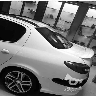
\includegraphics[width=0.8\linewidth]{../assets/sample_gray.png}\\{\scriptsize a real 206}
    \end{center}\end{column}
    \begin{column}{0.5\textwidth}\begin{center}
      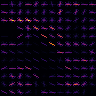
\includegraphics[width=0.8\linewidth]{../assets/hog_vis.png}\\{\scriptsize its HOG (edge-orientation) map}
    \end{center}\end{column}
  \end{columns}
  \vspace{2pt}
  HOG divides the image into \term{cells} and, in each, histograms the gradient directions — a compact shape signature.
\end{frame}

\begin{frame}{The HOG algorithm, step by step}
  \begin{enumerate}
    \item Compute gradients $I_x,I_y$ at every pixel.
    \item Get magnitude and orientation per pixel.
    \item Split the image into small \term{cells} (e.g.\ $8\times8$ px).
    \item In each cell, build a $9$-bin \term{histogram} of orientations, weighted by magnitude.
    \item Group cells into \term{blocks} and \term{normalize} (for lighting invariance).
    \item Concatenate all block histograms $\rightarrow$ one long feature vector.
  \end{enumerate}
  \keyidea{Steps 1--2 are last week's gradients. Steps 3--6 are what makes it a robust, fixed-length descriptor.}
\end{frame}

\begin{frame}{A worked HOG cell}
  \begin{columns}[T]
    \begin{column}{0.42\textwidth}
      One $2\times2$ patch of orientations (degrees), all magnitude $=1$ for simplicity:
      \[ \pixelgrid{{10,50},{50,130}} \]
      Bin width $20^\circ$, bins centred at $10,30,\dots,170$.
    \end{column}
    \begin{column}{0.58\textwidth}
      Votes into the $9$-bin histogram:
      \begin{center}
      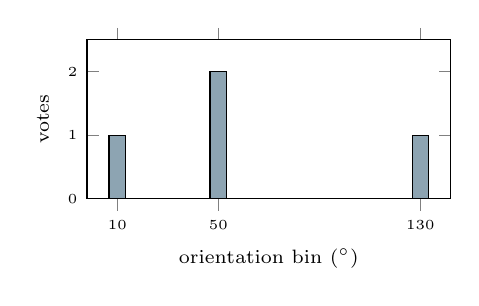
\begin{tikzpicture}
        \begin{axis}[width=6.2cm,height=3.6cm,ybar,bar width=6pt,
            ymin=0,ymax=2.5,xtick={10,50,130},
            xlabel={\scriptsize orientation bin ($^\circ$)},
            ylabel={\scriptsize votes},
            xlabel style={font=\scriptsize},ylabel style={font=\scriptsize},
            tick label style={font=\tiny}]
          \addplot[fill=coursePrimary!50] coordinates {(10,1)(50,2)(130,1)};
        \end{axis}
      \end{tikzpicture}
      \end{center}
      Two pixels point at $50^\circ$, so that bin gets $2$. The result is a $9$-number signature for this cell.
    \end{column}
  \end{columns}
\end{frame}

\begin{frame}{Block normalization — why it matters}
  \begin{columns}[T]
    \begin{column}{0.56\textwidth}
      \begin{itemize}
        \item Raw histogram values scale with \emph{contrast}: a sunny photo has bigger gradients everywhere.
        \item Group nearby cells into a \term{block} and divide by the block's norm.
        \item Now the descriptor depends on edge \emph{directions}, not on absolute brightness.
      \end{itemize}
    \end{column}
    \begin{column}{0.44\textwidth}
      \begin{mathbox}
        $L2$ normalization: $\displaystyle v \leftarrow \frac{v}{\sqrt{\lVert v\rVert^2 + \epsilon}}$.
        The tiny $\epsilon$ avoids dividing by zero in flat regions.
      \end{mathbox}
    \end{column}
  \end{columns}
  \begin{goodbox}
    Overlapping blocks (each cell counted in several blocks) is what makes real HOG robust to lighting.
  \end{goodbox}
\end{frame}

\begin{frame}{Why HOG works for shape}
  \begin{itemize}
    \item Cars differ in \emph{shape} (roofline, lights, grille) — captured by gradient directions.
    \item Histogramming per cell gives tolerance to small shifts and lighting changes.
    \item HOG + linear SVM was the state of the art for pedestrian/vehicle detection for years.
  \end{itemize}
  \keyidea{HOG throws away exact pixel values and keeps \emph{where edges point} — the essence of shape.}
\end{frame}

\begin{frame}{HOG hyper-parameters}
  \begin{center}
  \begin{tabular}{@{}lll@{}}
    \toprule
    \textbf{Knob} & \textbf{Typical} & \textbf{Effect} \\
    \midrule
    Cell size & $8\times8$ px & smaller $=$ finer detail, longer vector \\
    Orientation bins & $9$ & more bins $=$ finer angles, more noise \\
    Block size & $2\times2$ cells & bigger $=$ stronger normalization \\
    Signed angles? & no ($0$--$180^\circ$) & unsigned is usual for object shape \\
    \bottomrule
  \end{tabular}
  \end{center}
  \begin{infobox}[Vector length]
    A $96\times96$ image, $8\times8$ cells, $2\times2$ blocks, $9$ bins $\Rightarrow$ roughly $900$ numbers — the ``$900$-D'' vectors we train on.
  \end{infobox}
\end{frame}

% ==================================================================
\section{Beyond HOG}
% ==================================================================

\begin{frame}{Colour histograms — a complementary feature}
  \begin{columns}[T]
    \begin{column}{0.56\textwidth}
      \begin{itemize}
        \item HOG is grayscale — it ignores colour entirely.
        \item Some car models cluster around typical colours; a \term{colour histogram} captures that.
        \item Count pixels per colour bin (e.g.\ hue), normalize by pixel count.
      \end{itemize}
      Concatenate HOG $+$ colour to get a richer vector.
    \end{column}
    \begin{column}{0.44\textwidth}
      \begin{center}
      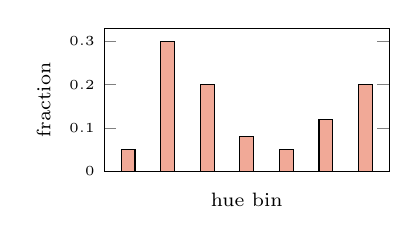
\begin{tikzpicture}
        \begin{axis}[width=5.2cm,height=3.4cm,ybar,bar width=5pt,ymin=0,
            xlabel={\scriptsize hue bin},ylabel={\scriptsize fraction},
            xlabel style={font=\scriptsize},ylabel style={font=\scriptsize},
            tick label style={font=\tiny},xtick=\empty]
          \addplot[fill=courseAccent!60] coordinates
            {(1,0.05)(2,0.30)(3,0.20)(4,0.08)(5,0.05)(6,0.12)(7,0.20)};
        \end{axis}
      \end{tikzpicture}
      \end{center}
    \end{column}
  \end{columns}
\end{frame}

\begin{frame}{Other classical descriptors}
  \begin{center}
  \begin{tabular}{@{}lll@{}}
    \toprule
    \textbf{Descriptor} & \textbf{Captures} & \textbf{Good for} \\
    \midrule
    HOG & edge orientations & overall shape \\
    LBP & local texture patterns & surface/texture, faces \\
    Colour hist. & colour distribution & colour-distinct classes \\
    ORB / SIFT & keypoints \& matches & alignment, stitching \\
    \bottomrule
  \end{tabular}
  \end{center}
  \keyidea{There is no single best feature. You pick (or combine) descriptors that expose what separates \emph{your} classes.}
\end{frame}

% ==================================================================
\section{What a classifier is}
% ==================================================================

\begin{frame}{What a classifier learns}
  \begin{itemize}
    \item Given feature vectors with labels, it learns a \term{decision boundary} between classes.
    \item \term{k-NN}: label a point by the majority vote of its $k$ nearest training points.
    \item \term{SVM}: find the boundary with the widest \term{margin} between classes.
  \end{itemize}
  \begin{mathbox}
    k-NN \emph{memorizes}; SVM \emph{optimizes} a margin. Both need features where classes are separable.
  \end{mathbox}
\end{frame}

\begin{frame}{k-NN in detail}
  \begin{columns}[T]
    \begin{column}{0.5\textwidth}
      \begin{itemize}
        \item ``Training'' just stores all labelled feature vectors.
        \item To predict: find the $k$ closest stored points, take a majority vote.
        \item Distance is usually Euclidean in feature space.
      \end{itemize}
      \begin{badbox}[Scale sensitivity]
        If one feature has a huge range, it dominates the distance. Standardize first.
      \end{badbox}
    \end{column}
    \begin{column}{0.5\textwidth}
      \begin{center}
      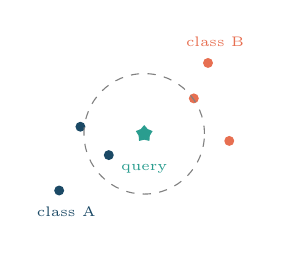
\begin{tikzpicture}[scale=0.9,font=\scriptsize]
        \fill[coursePrimary] (0.5,0.6) circle (2pt) (1.2,1.1) circle (2pt) (0.8,1.5) circle (2pt);
        \fill[courseAccent] (2.4,1.9) circle (2pt) (2.9,1.3) circle (2pt) (2.6,2.4) circle (2pt);
        \node[star,star points=5,fill=courseGood,inner sep=1.5pt] (q) at (1.7,1.4) {};
        \draw[dashed,gray] (1.7,1.4) circle (0.85);
        \node[coursePrimary] at (0.6,0.3) {\tiny class A};
        \node[courseAccent] at (2.7,2.7) {\tiny class B};
        \node[courseGood] at (1.7,0.9) {\tiny query};
      \end{tikzpicture}\\
      {\scriptsize $k{=}3$: nearest neighbours vote}
      \end{center}
    \end{column}
  \end{columns}
\end{frame}

\begin{frame}{A worked k-NN vote}
  \begin{columns}[T]
    \begin{column}{0.5\textwidth}
      Query at feature vector $q$. Distances to $5$ nearest training points:
      \begin{center}
      \begin{tabular}{@{}ccc@{}}
        \toprule
        neighbour & distance & label \\
        \midrule
        1 & 0.8 & 206 \\
        2 & 1.1 & 206 \\
        3 & 1.3 & Dena \\
        4 & 1.4 & 206 \\
        5 & 1.6 & 405 \\
        \bottomrule
      \end{tabular}
      \end{center}
    \end{column}
    \begin{column}{0.5\textwidth}
      \begin{itemize}
        \item With $k=5$: votes are 206$\times3$, Dena$\times1$, 405$\times1$.
        \item Majority $\Rightarrow$ predict \term{206}.
        \item With $k=1$ it would still be 206 (closest is 206).
      \end{itemize}
      \keyidea{Small $k$ = flexible but noisy; large $k$ = smooth but can wash out small classes.}
    \end{column}
  \end{columns}
\end{frame}

\begin{frame}{SVM \& the margin}
  \begin{columns}[T]
    \begin{column}{0.5\textwidth}
      \begin{itemize}
        \item An SVM finds the separating line with the \term{widest gap} to the nearest points.
        \item Those nearest points are the \term{support vectors}.
        \item A wide margin generalizes better than a boundary squeezed against the data.
        \item The \term{RBF kernel} lets the boundary curve for non-linear data.
      \end{itemize}
    \end{column}
    \begin{column}{0.5\textwidth}
      \begin{center}
      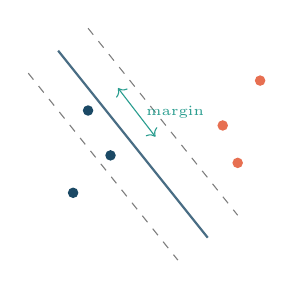
\begin{tikzpicture}[scale=0.95,font=\scriptsize]
        \fill[coursePrimary] (0.4,0.5) circle (2pt) (0.9,1.0) circle (2pt) (0.6,1.6) circle (2pt);
        \fill[courseAccent] (2.4,1.4) circle (2pt) (2.9,2.0) circle (2pt) (2.6,0.9) circle (2pt);
        \draw[thick,coursePrimary!80] (0.2,2.4) -- (2.2,-0.1);
        \draw[dashed,gray] (0.6,2.7) -- (2.6,0.2);
        \draw[dashed,gray] (-0.2,2.1) -- (1.8,-0.4);
        \draw[<->,courseGood] (1.0,1.9) -- (1.5,1.25) node[midway,right] {\tiny margin};
      \end{tikzpicture}
      \end{center}
    \end{column}
  \end{columns}
\end{frame}

\begin{frame}{Our classes in feature space (PCA to 2D)}
  \begin{center}
  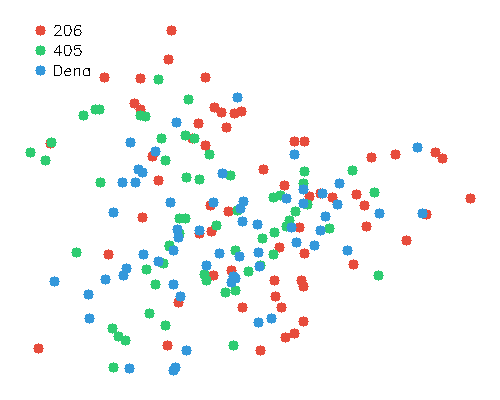
\includegraphics[width=0.5\linewidth]{../assets/feature_space.png}
  \end{center}
  \begin{itemize}
    \item Each dot is a real car's HOG vector, projected to 2D with PCA.
    \item Classes overlap a lot — these three models genuinely look similar. Hard problem!
  \end{itemize}
\end{frame}

\begin{frame}{Feature scaling — a quiet but critical step}
  \begin{columns}[T]
    \begin{column}{0.5\textwidth}
      \begin{goodbox}[Standardize]
        Rescale each feature to zero mean, unit variance \emph{before} k-NN or an RBF SVM.
      \end{goodbox}
    \end{column}
    \begin{column}{0.5\textwidth}
      \begin{badbox}[Leakage]
        Fit the scaler on \emph{training only}, then apply to test. Fitting on all data leaks test info.
      \end{badbox}
    \end{column}
  \end{columns}
  \keyidea{Distance-based methods are only as good as their scaling. HOG bins are already comparable, but mixing HOG with colour or size makes scaling essential.}
\end{frame}

% ==================================================================
\section{Train / test discipline}
% ==================================================================

\begin{frame}{Train / test split — the golden rule}
  \begin{itemize}
    \item Split data: \term{train} the classifier on one part, \term{test} on unseen data.
    \item Testing on training data lies — the model can just memorize.
    \item We used 70\% train / 30\% test, \term{stratified} (each class balanced in both).
  \end{itemize}
  \begin{badbox}
    Never report accuracy on data the model has seen. That number is meaningless for real use.
  \end{badbox}
\end{frame}

\begin{frame}{Stratification \& data leakage}
  \begin{columns}[T]
    \begin{column}{0.55\textwidth}
      \begin{itemize}
        \item \term{Stratified} split keeps each class's proportion in both train and test.
        \item Without it, a small class might vanish from the test set.
        \item \term{Leakage}: any test information sneaking into training inflates your score.
      \end{itemize}
    \end{column}
    \begin{column}{0.45\textwidth}
      \begin{infobox}[Common leaks]
        Scaling on all data, near-duplicate frames of the same car in both splits, tuning on the test set.
      \end{infobox}
    \end{column}
  \end{columns}
\end{frame}

% ==================================================================
\section{In-class exercise}
% ==================================================================

\begin{frame}{\faPen~In-class exercise (10 min)}
  \begin{infobox}[Design the features]
  \end{infobox}
  \begin{enumerate}
    \item A pixel has $I_x=30,\ I_y=40$. Give its gradient magnitude and (roughly) its orientation.
    \item You must separate white 206s from black 405s. Which feature helps most — HOG or colour? Why?
    \item Your HOG vector is $900$-D but you have $126$ training images. Name one risk and one fix.
  \end{enumerate}
\end{frame}

\begin{frame}{\faPen~Debrief}
  \begin{itemize}
    \item (1) Magnitude $=\sqrt{30^2+40^2}=50$; orientation $=\arctan(40/30)\approx 53^\circ$.
    \item (2) \term{Colour histograms} — the models differ mainly by colour here, and HOG is grayscale. Best: combine both.
    \item (3) Far more dimensions than samples $\Rightarrow$ overfitting risk; fix with PCA / fewer HOG cells / more data.
  \end{itemize}
  \keyidea{Choosing the right feature is half the battle — before any classifier is trained.}
\end{frame}

% ==================================================================
\section{Wrap-up}
% ==================================================================

\begin{frame}{Session 1 — what you can now do}
  \begin{itemize}
    \item Explain why raw pixels are a poor representation, and what makes a feature good.
    \item Compute a gradient's magnitude and orientation, and describe the HOG pipeline end to end.
    \item Combine HOG with colour or texture descriptors when needed.
    \item Describe k-NN and SVM, and set up a correct stratified train/test split.
  \end{itemize}
\end{frame}

\begin{frame}{Next session}
  \begin{alertblock}{Session 2 — training \& the truth about scores}
    \begin{itemize}
      \item Actually train k-NN and SVM in code on \code{E:/data}.
      \item Read our real results — and discover a $100\%$ train / $48\%$ test gap.
      \item Overfitting, confusion matrices, precision/recall, and cross-validation.
      \item Why hand-crafted features hit a ceiling — the doorway to deep learning.
    \end{itemize}
  \end{alertblock}
  No deliverable yet — bring your feature-extraction code from today.
\end{frame}

\begin{frame}[standout]
  Good features come first.\\[4pt]
  \normalsize A classifier can only draw a boundary in the space your features give it —
  next session we train one and see how honest it really is.
\end{frame}

\end{document}
